\documentclass[tikz,border=12pt]{standalone}

\usepackage{tikz}
\usepackage{xcolor}
\usepackage{fontspec}

% base6 — Constructivist Logo
\definecolor{LogoRed}{HTML}{D91E18}
\definecolor{LogoBlue}{HTML}{2364A3}
\definecolor{LogoYellow}{HTML}{F2B91F}
\definecolor{LogoGray}{HTML}{9A9A9A}
\definecolor{LogoBlack}{HTML}{101010}

\begin{document}
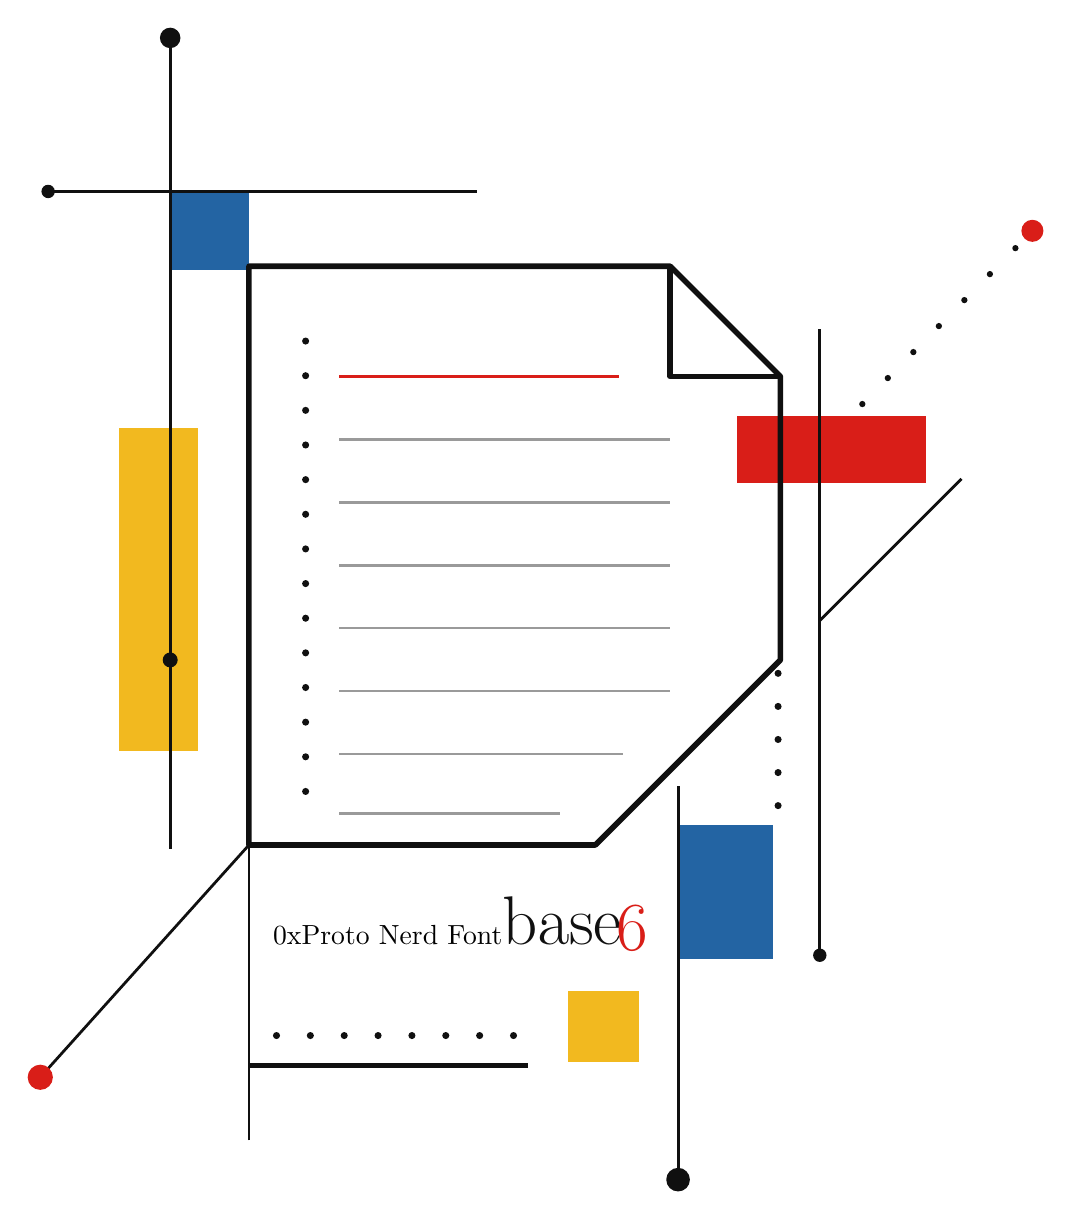
\begin{tikzpicture}[
    x=1cm,
    y=1cm,
    line cap=butt,
    line join=round
]

% Color blocks
\fill[LogoBlue] (2.0,10.2) rectangle (3.0,11.2);
\fill[LogoYellow] (1.35,4.1) rectangle (2.35,8.2);
\fill[LogoRed] (9.2,7.5) rectangle (11.6,8.35);
\fill[LogoBlue] (8.45,1.45) rectangle (9.65,3.15);
\fill[LogoYellow] (7.05,0.15) rectangle (7.95,1.05);

% Main page
\draw[LogoBlack, line width=2pt]
    (3.0,2.9) -- (3.0,10.25) -- (8.35,10.25) -- (9.75,8.85)
    -- (9.75,5.25) -- (7.40,2.90) -- cycle;
\draw[LogoBlack, line width=2pt]
    (8.35,10.25) -- (8.35,8.85) -- (9.75,8.85);

% Note lines
\draw[LogoRed, line width=1.1pt] (4.15,8.85) -- (7.70,8.85);
\foreach \y in {8.05,7.25,6.45,5.65,4.85}{
    \draw[LogoGray, line width=.75pt] (4.15,\y) -- (8.35,\y);
}
\draw[LogoGray, line width=.75pt] (4.15,4.05) -- (7.75,4.05);
\draw[LogoGray, line width=.75pt] (4.15,3.30) -- (6.95,3.30);

% Page dot column
\foreach \y in {9.30,8.86,8.42,7.98,7.54,7.10,6.66,6.22,5.78,5.34,4.90,4.46,4.02,3.58}{
    \fill[LogoBlack] (3.72,\y) circle (0.045);
}

% Left construction axes
\draw[LogoBlack, line width=1pt] (2.0,12.4) -- (2.0,2.85);
\draw[LogoBlack, line width=1pt] (0.45,11.2) -- (5.9,11.2);
\fill[LogoBlack] (2.0,13.15) circle (0.13);
\draw[LogoBlack, line width=1pt] (2.0,13.02) -- (2.0,12.40);
\fill[LogoBlack] (0.45,11.2) circle (0.085);
\fill[LogoBlack] (2.0,5.25) circle (0.095);

% Lower construction
\draw[LogoBlack, line width=1pt] (3.0,-0.85) -- (3.0,2.9);
\draw[LogoBlack, line width=1pt] (0.35,-0.05) -- (3.0,2.90);
\fill[LogoRed] (0.35,-0.05) circle (0.16);
\draw[LogoBlack, line width=2pt] (3.0,0.10) -- (6.55,0.10);
\foreach \x in {3.35,3.78,4.21,4.64,5.07,5.50,5.93,6.36}{
    \fill[LogoBlack] (\x,0.48) circle (0.045);
}

% Right construction
\draw[LogoBlack, line width=1pt] (10.25,1.5) -- (10.25,9.45);
\draw[LogoBlack, line width=1pt] (10.25,5.75) -- (12.05,7.55);
\foreach \t in {0.20,0.32,0.44,0.56,0.68,0.80,0.92}{
    \fill[LogoBlack] ({10.25 + 2.70*\t},{7.95 + 2.75*\t}) circle (0.04);
}
\fill[LogoRed] (12.95,10.70) circle (0.14);
\foreach \y in {3.4,3.82,4.24,4.66,5.08}{
    \fill[LogoBlack] (9.72,\y) circle (0.045);
}
\fill[LogoBlack] (10.25,1.5) circle (0.085);

% Blue vertical axis
\draw[LogoBlack, line width=1.1pt] (8.45,-1.35) -- (8.45,3.65);
\fill[LogoBlack] (8.45,-1.35) circle (0.15);

% base6 wordmark
\node[anchor=west, inner sep=0pt] at (3.30,1.90){
    \fontspec{0xProto Nerd Font}\fontsize{31}{31}\selectfont
    \textcolor{LogoBlack}{base}%
    \kern-0.08em%
    \raisebox{-0.20ex}{%
        \fontsize{30}{30}\selectfont
        \textcolor{LogoRed}{6}%
    }
};

\end{tikzpicture}
\end{document}
